\documentclass{article}
\usepackage[utf8]{inputenc}
\usepackage{hyperref,ragged2e,amsmath,multicol,gensymb,setspace,
fancyhdr,amsfonts,tikz,pgfplots,nccmath,enumerate,verbatim}
\usepackage[a4paper, width=216mm, height=297mm, margin=3cm]{geometry}
\usepgfplotslibrary{polar,fillbetween}
\usepgflibrary{shapes.geometric}
\usetikzlibrary{calc,patterns,arrows}
\newcommand\mylog[1]{\mathop{{}^{#1}\mathrm{log}}}
\pgfplotsset{compat=1.15}
\pgfplotsset{my style/.append style={axis x line=middle, axis y line=
middle, xlabel={$x$}, ylabel={$y$}, axis equal }}
\usepackage{etoolbox}
\newcommand{\zerodisplayskips}{%
  \setlength{\abovedisplayskip}{0pt}%
  \setlength{\belowdisplayskip}{0pt}%
  \setlength{\abovedisplayshortskip}{0pt}%
  \setlength{\belowdisplayshortskip}{0pt}}
\pagestyle{fancy}
\fancyhf{}
\lhead{Halaman \thepage}
\rhead{Pembahasan Soal EAS 2020/2021 \\ (\href{https://instagram.com/ahmadzakiyudin_/}{@ahmadzakiyudin\_})}
\hypersetup{
    colorlinks=true,
    linkcolor=blue,
    filecolor=blue,      
    urlcolor=blue,
}
\setlength{\columnsep}{0.8cm}
\begin{document}
 \begin{titlepage}
    \vspace*{\fill}
    \begin{center}
      \Huge {PEMBAHASAN SOAL EAS \\ MATEMATIKA I \\ TAHUN 2020/2021}\\[0.4 cm]
      \huge {Ahmad Hisbu Zakiyudin}
    \end{center}
    \vspace*{\fill}
  \end{titlepage}
\makeatletter
\renewcommand*\env@matrix[1][*\c@MaxMatrixCols c]{%
  \hskip -\arraycolsep
  \let\@ifnextchar\new@ifnextchar
  \array{#1}}
\makeatother
\newcount\arrowcount
\newcommand\arrows[1]{
        \global\arrowcount#1
        \ifnum\arrowcount>0
                \begin{matrix}[c]
                \expandafter\nextarrow
        \fi
}

\newcommand\nextarrow[1]{
        \global\advance\arrowcount-1
        \ifx\relax#1\relax\else \xrightarrow{#1}\fi
        \ifnum\arrowcount=0
                \end{matrix}
        \else
                \\
                \expandafter\nextarrow
        \fi
}
\newpage
\setstretch{1.3}
\section*{SOAL SESI 1}
\begin{enumerate}
	\item Diberikan $y=f(x)=\dfrac{x+3}{x+2}$
	\begin{enumerate}
		\item Dapatkan $y'=f'(x)$
		\item Jika $(x_0,y_0)$ titik pada kurva $f$ dimana garis singgung dari $f$ tegak lurus dengan garis $y=x$, maka tentukan titik $(x_0,y_0)$ dan persamaan garis singgung di titik tersebut.
	\end{enumerate}
	\textbf{Solusi:}
	\begin{enumerate}
		\item Dapat dengan mudah diperoleh $y'=f'(x)=\dfrac{(x+2)(1)-(x+3)(1)}{(x+2)^2} = -\dfrac{1}{(x+2)^2}$
		\item Ingat bahwa gradien garis singgung kurva pada suatu titik pada kurva adalah nilai turunan pertama pada titik tersebut. Tinjau bahwa gradien garis singgung yang dimaksud tegak lurus dengan garis $y=x$ sehingga gradien garis singgungnya adalah $-1$. Selanjutnya kita cari nilai $x$ yang memenuhi $f'(x)=-1$
		\begin{align*}
		f'(x) = -\dfrac{1}{(x+2)^2} &= -1 \\
		(x+2)^2 &=1\\
		|x+2| &= 1 
		\end{align*}
		sehingga terdapat dua titik $x_0$ yang memenuhi, yaitu $x_0=-3$ dan $x_0=-1$. 
		\begin{enumerate}
			\item Untuk $x_0=-3$ kita peroleh $y_0=f(x_0)=f(-3)=0$ sehingga persamaan garis singgung di titik tersebut adalah 
			\begin{align*}
			y-y_0 &= m(x-x_0) \\
			y &= -1(x-(-3)) \\
			y &= -x-3 \\
			x+y +3&= 0
			\end{align*}
			\item Untuk $x_0=-1$, kita peroleh $y_0=f(x_0)=f(-1)=2$ sehingga persamaan garis singgung di titik tersebut adalah 
			\begin{align*}
			y-y_0 &= m(x-x_0)\\
			y-2 &= -1(x-(-1)) \\
			y &= -x+1 \\
			x+y-1 &= 0
			\end{align*}
		\end{enumerate}
		Jadi terdapat dua titik $(x_0,y_0)$ pada kurva $f(x)$ yang garis singgungnya tegak lurus dengan garis $y=x$, yaitu titik $(-3,0)$ dengan garis singgung $x+y+3=0$ dan titik $(-1,2)$ dengan garis singgung $x+y-1=0$
	\end{enumerate}
	\newpage 
	\item Diketahui $f'(x)=\sqrt{3x+4}$ dan $g(x)=x^2-1$. Didefinisikan $F(x)=f(g(x))$, dapatkan $F'(x)$\\
	\textbf{Solusi:}\\
	Untuk mendapatkan $F'(x)$ ingat kembali aturan rantai
	\begin{align*}
	F'(x) =f'(g(x))g'(x) = g'(x)\sqrt{3g(x)+4} = 2x\sqrt{3x^2+1}
	\end{align*}
	\item Tentukan nilai maksimum dan minimum dari fungsi $f(x)=\begin{cases} 4x-2, &x<1 \\
	(x-2)(x-3), &x\geq 1\end{cases}$ pada $\left[\frac{1}{2},\frac{7}{2}\right]$
	\\[0.1 cm] \textbf{Solusi:}\\
	Akan kita cari masing-masing nilai maksimum dan minimum $f(x)$ pada selang $\left[\frac{1}{2},1\right)$ dan $\left[1,\frac{7}{2}\right]$
	\begin{enumerate}
		\item[i.] Untuk selang $\left[\frac{1}{2},1\right)$, diperoleh $f(x)=4x-2$ dan $f'(x)=4$, sehingga $f'(x)>0$ untuk setiap $x$ pada selang tersebut, serta $f(x)$ tidak memiliki titik stasioner. Oleh karena itu, dapat dicek pada batas selangnya, yaitu $f\left(\frac{1}{2}\right)=0$ adalah nilai minimum. Sedangkan nilai maksimumnya tidak ada, tetapi mendekati $\displaystyle \lim_{x\rightarrow 1^-} 4x-2 = 2$.
		\item[ii.] Untuk selang $\left[1,\frac{7}{2}\right]$, diperoleh $f(x)=(x-2)(x-3)=x^2-5x+6$ dan $f'(x)=2x-5$. Dapat diperoleh pula $f''(x)=2$ sehingga $f''\left(\frac{5}{2}\right)=2>0$, artinya $x=\dfrac{5}{2}$ merupakan nilai minimum relatif. Selanjutnya dapat dicek nilai $f(x)$ pada batas selang dan titik stasioner 
		\begin{align*}
		f(1)&=(1-2)(1-3)=2 \\
		f\left(\frac{5}{2}\right) &=\left(\frac{5}{2}-2\right)\left(\frac{5}{2}-3\right) = -\frac{1}{4} \\
		f\left(\frac{7}{2}\right) &= \left(\frac{7}{2}-2\right)\left(\frac{7}{2}-3\right) = \frac{3}{4}
		\end{align*}
		sehingga nilai minimum pada selang $\left[1,\frac{7}{2}\right]$ adalah $f\left(\frac{5}{2}\right) = -\frac{1}{4}$ dan maksimum adalah $f(1)=2$
	\end{enumerate}
	Apabila kedua hasil tersebut digabungkan, dapat diperoleh nilai maksimum dan minimum global berturut-turut $f(1)=2$ dan $f\left(\frac{5}{2}\right) = -\frac{1}{4}$. Selain itu, diperoleh pula maksimum relatif dan minimum relatif berturut-turut $f\left(\frac{7}{2}\right)=\frac{3}{4}$ dan $f\left(\frac{1}{2}\right)=0$
	\item Terdapat dua Kilang minyak lepas pantai, Kilang 1 berjarak 3 km dan Kilang 2 berjarak 4 km dari daratan, jarak Kilang 1 dan Kilang 2 adalah 5 km. Akan dibangun Tangki untuk menampung hasil kilang. Tangki terletak di daratan antara Kilang 1 dan Kilang 2 (lihat gambar). Tentukan letak Tangki dengan jarak minimum dari Kilang 1 dan Kilang 2.
	\begin{center}
	\begin{tikzpicture}[scale = 0.43]
	\draw[thick] (-2,0) -- (12,0);
	\draw[thick,blue,latex-latex] (0,0.1) -- (0,6);
	\draw[thick,blue,latex-latex] (10,0.1) -- (10,8);
	\draw[thick,blue,latex-latex] (0,-0.3) -- (10, -0.3);
	\draw (10,8) node[above] {\includegraphics[scale=0.12]{kilang.png}};
	\draw (9,8.5)  node[left] {\large{$K_2$}};
	\draw (0,6) node[above] {\includegraphics[scale=0.12]{kilang.png}};
	\draw (-1,6.5)  node[left] {\large{$K_1$}};
	\draw (0,3) node[left] {3 km};
	\draw (10,4) node[right] {4 km};
	\draw (5,-0.3) node[below] {5 km};
	\draw (5.8,-0.2) node[above] {\includegraphics[scale=0.5]{tangki.png}~Tangki};
	\end{tikzpicture}
\end{center}
	\textbf{Solusi:}\\
	Misalkan terdapat $P_1$ dan $P_2$ di daratan sehingga sehingga $P_1K_1=3$ km dan $P_2K_2=4$ km merupakan jarak antara Kilang 1 dan Kilang 2 ke daratan, akibatnya $P_1P_2=5$ km. Selanjutnya misalkan Tangki berada di titik $T$ dan $P_1T=x$, sehingga $P_2T=5-x$. Oleh karena itu, dapat diperoleh jarak antara Kilang 1 dengan Tangki adalah $K_1T=\sqrt{K_1P_1+P_1T^2}=\sqrt{x^2+9}$, serta jarak antara Kilang 2 dengan Tangki adalah $K_2T=\sqrt{K_2P_2+P_2T} = \sqrt{16+(5-x)^2}$. Karena kita perlu mencari jarak minimum $K_1T$ dan $K_2T$ sekaligus, maka jika kita jumlahkan jarak keduanya, pasti minimum juga. Misalkan jumlah jarak keduanya adalah $y=\sqrt{x^2+9}+\sqrt{16+(5-x)^2}$, maka minimumnya adalah titik $x$ saat $\dfrac{dy}{dx} = 0$ yaitu
	\begin{align*}
	\dfrac{dy}{dx} = \dfrac{2x}{2\sqrt{x^2+9}} + \dfrac{2(5-x)(-1)}{2\sqrt{16+(5-x)^2}} &= 0\\
	\dfrac{x\sqrt{x^2-10x+41}+(x-5)\sqrt{x^2+9}}{\sqrt{x^2+9}\sqrt{x^2-10x+41}} &= 0\\
	x\sqrt{x^2-10x+41}+(x-5)\sqrt{x^2+9} &= 0\\
	x\sqrt{x^2-10x+41} &= (5-x)\sqrt{x^2+9} \\
	x^2(x^2-10x+41) &= (x^2-10x+25)(x^2+9)\\
	x^4-10x^3+41x^2 &= x^4+9x^2-10x^3-90x+25x^2+225 \\
	7x^2+90x-225 &= 0\\
	(x+15)(7x-15) &= 0 
	\end{align*}
	Karena $0<x<5$, maka $x=\dfrac{15}{7}$. Jadi jarak minimum Kilang 1 dengan Tangki adalah $$K_1T=\sqrt{9+x^2}=\sqrt{9+\left(\frac{15}{7}\right)^2}=\dfrac{3}{7}\sqrt{74} \text{ km}$$
	serta jarak minimum Kilang 2 dengan Tangki adalah $$K_2T=\sqrt{16+(5-x)^2} = \sqrt{16+\left(5-\frac{15}{7}\right)^2} = \dfrac{4}{7}\sqrt{74} \text{ km}$$
	\item Tentukan nilai integral berikut
	\begin{enumerate}
		\item $\displaystyle \int_0^2 |3x-2| \, dx$
		\item $\displaystyle \int_{\frac{1}{2}}^1 \dfrac{1}{x^2}f\left(\dfrac{1}{x}\right) \, dx$ jika $\displaystyle \int_1^2 f(x) \, dx =3$
	\end{enumerate}
	\textbf{Solusi:}
	\begin{enumerate}
		\item Tinjau bahwa $|3x-2| = \begin{cases} 3x-2, &x\geq\frac{2}{3}\\
		2-3x, &x<\frac{2}{3} \end{cases}$ sehingga 
		\begin{align*}
		\int_0^2 |3x-2| \, dx &= \int_0^{\frac{2}{3}} (2-3x) \, dx + \int_{\frac{2}{3}}^2 (3x-2) \, dx \\
		&= \left[2x-\dfrac{3x^2}{2}\right]^{\frac{2}{3}}_0 + \left[\dfrac{3x^2}{2}-2x\right]_{\frac{2}{3}}^2\\
		&= \frac{10}{3}
		\end{align*}
		\item Misalkan $u = \dfrac{1}{x}$ sehingga $du = -\dfrac{1}{x^2} \, dx$. \\Batas atas integral menjadi $u=\dfrac{1}{1}=1$ dan batas bawahnya menjadi $u=\dfrac{1}{\frac{1}{2}}=2$. Pada soal diketahui bahwa $\displaystyle \int_1^2 f(x)\, dx =3$ sehingga 
		\begin{align*}
		\int_{\frac{1}{2}}^1 \dfrac{1}{x^2}f\left(\frac{1}{x}\right) \, dx &= \int_2^1 -f(u) \, du\\
		&= -\int_2^1 f(u) \,du\\
		&= \int_1^2 f(u) \, du \\
		&= 3
		\end{align*}
	\end{enumerate}
\end{enumerate}
\newpage
\section*{SOAL SESI 2}
\begin{enumerate}
	\item Dapatkan $\dfrac{dy}{dx}$ dari $x^3y^2-3xy^2+x+y\sin x =5$
	\\[0.1 cm] \textbf{Solusi:}\\
	Ingat kembali aturan perkalian dan aturan rantai pada turunan, serta sifat-sifat turunan dan turunan fungsi implisit. Turunkan kedua ruas terhadap $x$, diperoleh
	\begin{align*}
	\dfrac{d}{dx}[x^3y^2-3xy^2+x+y\sin x] &= \dfrac{d}{dx}[5] \\
	\dfrac{d}{dx}[x^3y^2]-\dfrac{d}{dx}[3xy^2]+\dfrac{d}{dx}[x] +\dfrac{d}{dx}[y\sin x] &= \dfrac{d}{dx} [5] \\
	3x^2y^2+2x^3y\dfrac{dy}{dx}-\left(3y^2+6xy\dfrac{dy}{dx}\right) + 1 + \sin x\dfrac{dy}{dx} +y\cos x &= 0 \\
	3x^2y^2-3y^2+y\cos x+1 + \left(2x^3y-6xy+\sin x\right)\dfrac{dy}{dx} &= 0 \\
	\left(2x^3y-6xy+\sin x\right)\dfrac{dy}{dx} &= 3y^2-3x^2y^2-y\cos x -1 \\
	\dfrac{dy}{dx} &= \dfrac{3y^2(1-x^2)-y\cos x -1}{2xy(x^2-3)+\sin x}
	\end{align*}
	\item Tentukan semua titik pada kurva $y^2-x^2+5=0$ yang terdekat ke titik $(0,4)$
	\\[0.1 cm] \textbf{Solusi:}\\
	Tinjau persamaan jarak titik $x$ ke $0$ dan titik $y$ ke $4$ yaitu $P=\sqrt{x^2+(y-4)^2}$. Diketahui pula bahwa $y^2-x^2+5=0$ sehingga $P=\sqrt{y^2+5+(y-4)^2}$. Untuk mencari jarak terdekat, kita gunakan turunan, dan supaya mudah dapat dicari turunan dari $P^2=2y^2-8y+21$ terhadap $y$ yang bernilai 0, sehingga 
	 \begin{align*}
	 \dfrac{dP^2}{dy} &= 4y-8 = 0 \\
	 y &= 2
	 \end{align*}
	 Karena $y=2$, maka $x=\pm 3$. Dengan demikian, titik pada kurva $y^2-x^2+5=0$ dengan jarak terdekat ke $(0,4)$ adalah titik $(-3,2)$ dan $(3,2)$ dengan jarak $P=\sqrt{3^2+(2-4)^2}=\sqrt{13}$
	 \item Diketahui $f(x)=6x^{\frac{1}{3}}-3x^{\frac{4}{3}}$
	 \begin{enumerate}
	 	\item Dengan uji turunan pertama, periksa titik kritisnya dan jenis maksimum-minimumnya
	 	\item Dengan uji turunan kedua, periksa titik beloknya
	 	\item Sketsa grafik fungsi tersebut.
	 \end{enumerate}
	 \textbf{Solusi:}
	 \begin{enumerate}
	 	\item Tinjau $f'(x)=2x^{-\frac{2}{3}}-4x^{\frac{1}{3}}=\dfrac{2}{\sqrt[3]{x^2}}-4\sqrt[3]{x}=\dfrac{2-4x}{\sqrt[3]{x^2}}$. Selanjutnya, untuk menentukan titik kritis, yaitu nilai $x$ sehingga pembilang bernilai 0 atau penyebut bernilai 0. Saat pembilang bernilai nol, yaitu titik stasioner adalah $x=\dfrac{1}{2}$. Sedangkan saat penyebut bernilai 0, yaitu ketika $x=0$ adalah titik singular. Perhatikan bahwa tanda $f'(x)$ berubah dari positif ke negatif di $x=\dfrac{1}{2}$ dan hanya titik tersebut yang merupakan titik stasioner, sehingga $f\left(\frac{1}{2}\right)=\dfrac{9}{2\sqrt[3]{2}}$ adalah maksimum global.
	 	\item Untuk mendapatkan titik belok, tinjau $f''(x)=-\dfrac{4}{3}x^{-\frac{5}{3}}-\dfrac{4}{3}x^{-\frac{2}{3}}=-\dfrac{4}{3\sqrt[3]{x^2}}\left(\dfrac{1}{x}+1\right)$. Dapat dengan mudah diperoleh bahwa $x=0$ dan $x=-1$ merupakan titik kritis dari $f'(x)$. Perhatikan bahwa $f''(x)<0$ pada selang $(-\infty,-1)\cup (0,+\infty)$ sehingga $f(x)$ cekung ke bawah pada selang tersebut, serta $f''(x)>0$ pada selang $(-1,0)$ sehingga $f(x)$ cekung ke atas pada selang tersebut. Karena terjadi perubahan kecekungan pada $x=-1$ dan $x=0$, maka titik $(-1,f(-1))=(-1,-9)$ dan titik $(0,f(0))=(0,0)$ merupakan titik belok kurva $f(x)$.
	 	\item Sebelum menggambar sketsa grafik, cek titik potong dengan sumbu$-x$ dan sumbu$-y$. Titik potong dengan sumbu$-x$ saat $f(x)=3x^{\frac{1}{3}}(2-x)=0$, yaitu pada titik $x=0$ dan $x=2$. Titik potong dengan sumbu$-y$ saat $x=0$ yaitu titik $(0,0)$. Dapat diperoleh sketsa grafiknya adalah 
	 	\begin{center}
		\begin{tikzpicture}
		[
    declare function=
    {
      t(\x) = x/abs(x)*(abs(\x))^(1/3) ;
    }
  ]
\begin{axis}[
x =.9 cm, y=.7 cm,
 axis lines=middle,
  xmin=-3.5,xmax=5,ymin=-8,ymax=5,
  xtick distance=1,
  ytick distance=1,
  xlabel=$x$,
  ylabel=$y$]
\addplot [blue,domain=-1.3:3, samples=5000] {6*t(x)-3*t(x)^4};
\end{axis}

\end{tikzpicture}
		\end{center}
	 \end{enumerate}
	 \item Diketahui $f(x)=\dfrac{x}{x^2+2}$. Tentukan selang di mana $f(x)$
	 \begin{enumerate}
	 	\item Naik
	 	\item Turun
	 	\item Cekung ke bawah
	 	\item Cekung ke atas
	 	\item Tentukan nilai $x$ untuk semua titik belok
	 \end{enumerate}
	 \textbf{Solusi:}\\
	 Tinjau $f'(x)=\dfrac{x^2+2-x(2x)}{(x^2+2)^2}=\dfrac{(\sqrt{2}-x)(\sqrt{2}+x)}{(x^2+2)^2}$, maka $f'(x)=0$ ketika $x=-\sqrt{2}$ dan $x=\sqrt{2}$. Dapat diperoleh $f'(x)<0$ pada selang $(-\infty,-\sqrt{2})\cup (\sqrt{2},+\infty)$, serta $f'(x)>0$ pada selang $(-\sqrt{2},\sqrt{2})$. Selanjutnya tinjau $$ f''(x)=\dfrac{-2x(x^2+2)^2-(2-x^2)(2(x^2+2)(2x))}{(x^2+2)^4}=\dfrac{2x^3-12x}{(x^2+2)^3} = \dfrac{2x(x-\sqrt{6})(x+\sqrt{6})}{(x^2+2)^3} $$. Dapat diperoleh $f''(x)<0$ pada selang $(-\infty,-\sqrt{6})\cup (0,\sqrt{6})$ dan $f''(x)>0$ pada selang $(-\sqrt{6},0)\cup (\sqrt{6},+\infty)$
	 \begin{enumerate}
	 	\item Karena $f(x)$ kontinu, maka $f(x)$ naik pada selang $[-\sqrt{2},\sqrt{2}]$
	 	\item Karena $f(x)$ kontinu, maka $f(x)$ turun pada selang $(-\infty,-\sqrt{2}]\cup[\sqrt{2},+\infty)$
		\item $f(x)$ cekung ke bawah saat $f''(x)<0$, yaitu pada selang $(-\infty,-\sqrt{6})\cup (0,\sqrt{6})$	 	
	 	\item $f(x)$ cekung ke atas saat $f''(x)>0$, yaitu pada selang $(-\sqrt{6},0)\cup (\sqrt{6},+\infty)$
	 	\item Titik belok yaitu titik saat $f(x)$ berubah kecekungannya, yaitu saat $f''(x)=0$. Kita peroleh titik beloknya adalah $\left(-\sqrt{6},\frac{-\sqrt{6}}{8}\right)$, $(0,0)$, serta $\left(\sqrt{6},\frac{\sqrt{6}}{8}\right)$
	 \end{enumerate}
	 \item Dengan menggunakan rumus luas dari geometri bidang, hitunglah:
	 	\begin{enumerate}
	 		\item $\displaystyle \int_0^4 5-\sqrt{16-x^2} \, dx$
	 		\item $\displaystyle \int 5+\sqrt{8x-x^2} \, dx$
	 	\end{enumerate}
	 	\textbf{Solusi:}
	 	\begin{enumerate}
	 		\item Dengan sifat integral, kita punya $\displaystyle \int_0^4 5-\sqrt{16-x^2} \, dx = \int_0^4 5 \, dx- \int_0^4 \sqrt{16-x^2} \, dx$. Integral tersebut, dapat diinterpretasikan sebagai luas daerah di bawah kurva $y=5$ dikurangi dengan luas daerah di bawah kurva $y=\sqrt{16-x^2}$ dari 0 sampai 4. Tinjau bahwa $y=\sqrt{16-x^2}$ merupakan setengah lingkaran pada sumbu$-y$ positif dengan pusat $(0,0)$ dan jari-jari 4. Oleh karena itu, jika kita gambar daerahnya adalah 
	 		\begin{center}
	 		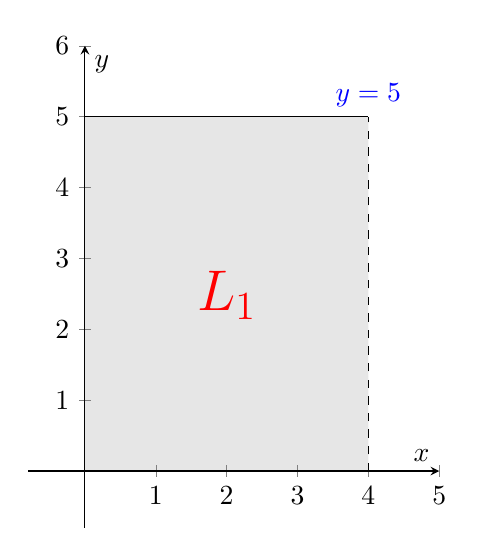
\begin{tikzpicture}
\begin{axis}[
x= 0.9 cm, y=0.9 cm,
 axis lines=middle,
  xmin=-0.8,xmax=5,ymin=-0.8,ymax=6,
  xtick distance=1,
  ytick distance=1,
  xlabel=$x$,
  ylabel=$y$]
\addplot [domain=0:4, name path=A] {5} node[above,blue] {$y=5$};
\addplot [domain=0:4, name path=B] {0};
\addplot[gray,opacity=0.2] fill between[of=B and A];
\draw[dashed] (4,0) -- (4,5);
\draw (2,2) node[red,above] {\huge{$L_1$}};
\end{axis}
\end{tikzpicture} \qquad
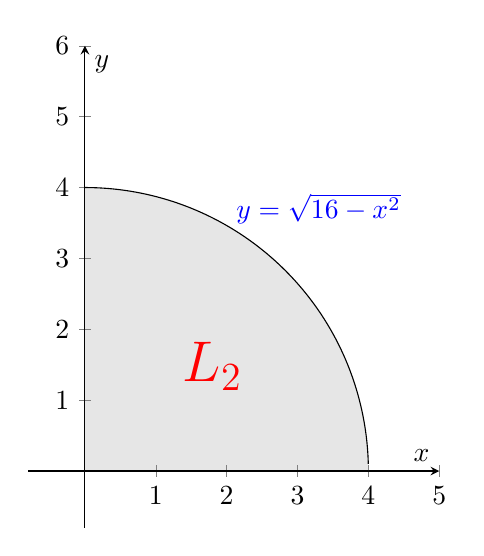
\begin{tikzpicture}
\begin{axis}[
x= 0.9 cm, y=0.9 cm,
 axis lines=middle,
  xmin=-0.8,xmax=5,ymin=-0.8,ymax=6,
  xtick distance=1,
  ytick distance=1,
  xlabel=$x$,
  ylabel=$y$]
\addplot [domain=0:4, name path=B,samples=3000] {sqrt(16-x^2)};
\addplot [domain=0:4, name path=A]{0};
\addplot[gray,opacity=0.2] fill between[of=B and A];
\draw (2,3.7) node[right,blue] {$y=\sqrt{16-x^2}$};
\draw (1.8,1) node[red, above] {\huge{$L_2$}};
\end{axis}
\end{tikzpicture}
	 		\end{center}
	 		Mudah terlihat bahwa $L_1$ merupakan persegi panjang dengan panjang 5 dan lebar 4 sehingga $L_1=5\times 4=20$ dan $L_2$ merupakan seperempat lingkaran dengan jari-jari $4$ sehingga $L_2=\dfrac{1}{4}\pi(4)^2=4\pi$. Dapat diperoleh hasil integralnya adalah $L_1-L_2=20-4\pi$.  
	 		\item Dengan sifat integral, kita punya $\displaystyle \int 5+\sqrt{8x-x^2} \, dx = \int 5 \, dx+ \int \sqrt{16-(x-4)^2} \, dx$. Integral tersebut, dapat diinterpretasikan sebagai luas daerah di bawah kurva $y=5$ ditambah dengan luas daerah di bawah kurva $y=\sqrt{16-(x-4)^2}$. Tinjau bahwa $y=\sqrt{16-(x-4)^2}$ merupakan setengah lingkaran pada sumbu$-y$ positif dengan pusat (4,0) dan jari-jari 4. Seharusnya, integral ini memiliki batas atas dan batas bawah, karena tidak diketahui dari soal, dapat diasumsikan batas bawah adalah 0 dan batas atasnya adalah 8, sehingga jika kita gambar daerahnya adalah 
	 		\begin{center}
	 		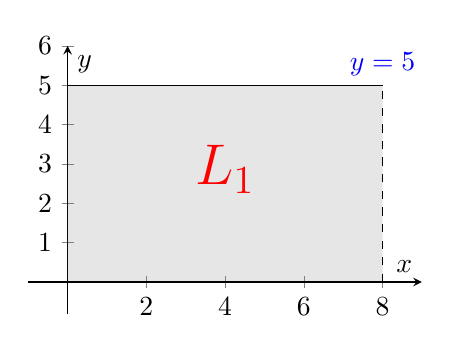
\begin{tikzpicture}
\begin{axis}[
x= 0.5 cm, y=0.5 cm,
 axis lines=middle,
  xmin=-1,xmax=9,ymin=-0.8,ymax=6,
  xtick distance=2,
  ytick distance=1,
  xlabel=$x$,
  ylabel=$y$]
\addplot [domain=0:8, name path=A] {5} node[above,blue] {$y=5$};
\addplot [domain=0:8, name path=B] {0};
\addplot[gray,opacity=0.2] fill between[of=B and A];
\draw[dashed] (8,0) -- (8,5);
\draw (4,2) node[red,above] {\huge{$L_1$}};
\end{axis}
\end{tikzpicture} \qquad
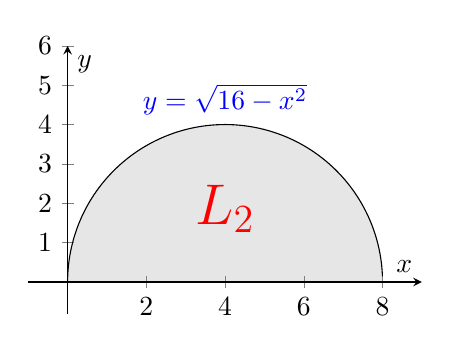
\begin{tikzpicture}
\begin{axis}[
x= 0.5 cm, y=0.5 cm,
 axis lines=middle,
  xmin=-1,xmax=9,ymin=-0.8,ymax=6,
  xtick distance=2,
  ytick distance=1,
  xlabel=$x$,
  ylabel=$y$]
\addplot [domain=0:8, name path=B,samples=3000] {sqrt(16-(x-4)^2)};
\addplot [domain=0:8, name path=A]{0};
\addplot[gray,opacity=0.2] fill between[of=B and A];
\draw (4,4) node[above,blue] {$y=\sqrt{16-x^2}$};
\draw (4,1) node[red, above] {\huge{$L_2$}};
\end{axis}
\end{tikzpicture}
	 		\end{center}
	 		Mudah terlihat bahwa $L_1$ merupakan persegi panjang dengan panjang 8 dan lebar 5 sehingga $L_1=8\times 5=40$ dan $L_2$ merupakan setengah lingkaran dengan jari-jari $4$ sehingga $L_2=\dfrac{1}{2}\pi(4)^2=8\pi$. Dapat diperoleh hasil integralnya adalah $L_1+L_2=40+8\pi$.
	 	\end{enumerate}
\end{enumerate}
\newpage
\section*{SOAL SESI 3}
\begin{enumerate}
	\item Diberikan fungsi sepotong-sepotong: $f(x) =\begin{cases} 3x-1; &x\geq 2 \\ x^2+1; &x<2\end{cases}$
	\begin{enumerate}
		\item Selidiki apakah $f(x)$ kontinu di $x=2$
		\item Selidiki apakah $f(x)$ diferensiabel (dapat diturunkan) di $x=2$
		\item Tentukan $f'(x)$
		\item Sketsa grafik $f(x)$ dan $f'(x)$
	\end{enumerate}
	\textbf{Solusi:}
	\begin{enumerate}
		\item $f(x)$ kontinu di titik $x=c$ jika dan hanya jika memenuhi tiga syarat, yaitu 
		\begin{enumerate}
			\item $f(c)$ ada, yaitu $f(2)=3(2)-1=5$
			\item $\displaystyle \lim_{x\rightarrow c} f(x) $ ada nilainya. \\Tinjau $\displaystyle \lim_{x\rightarrow 2} f(x) = \lim_{x\rightarrow 2^-} x^2+1 = 5$ dan $\displaystyle \lim_{x\rightarrow 2^+} f(x) = \lim_{x\rightarrow 2} 3x-1 = 5$ sehingga $\displaystyle \lim_{x\rightarrow 2} f(x) =\lim_{x\rightarrow 2^-} f(x)=\lim_{x\rightarrow 2^+} f(x) =5$
			\item $\displaystyle \lim_{x\rightarrow c} f(x) = f(c)$, yaitu $\displaystyle \lim_{x\rightarrow 2} f(x) = 5 = f(2)$
		\end{enumerate}
		Jadi $f(x)$ kontinu di $x=2$
		\item Dapat diturunkan di $x=c$ jika $f'_-(c)=f'_+(c)$\\
		Tinjau $f'_-(2)=2(2)=4$ dan $f'_+(2)=3$, sehingga $f(x)$ tidak dapat diturunkan di $x=2$
		\item Karena $f(x)$ tidak dapat diturunkan di $x=2$, maka $f(x)$ kita bagi menjadi dua selang yaitu untuk $x<2$ dan untuk $x>2$. Untuk $x<2$ diperoleh $f'(x)=2x$ sedangkan untuk $x>2$ diperoleh $f'(x)=3$, sehingga $f'(x)=\begin{cases}3; &x>2 \\ 2x; &x<2\end{cases}$
		\item Tinjau bahwa $f(x)$ untuk $x<2$ merupakan fungsi kuadrat yang digeser 1 satuan ke atas dan untuk $x\geq 2$ merupakan fungsi linear dengan gradien 3 dan digeser ke bawah sebanyak 1 satuan sehingga grafik fungsi $f(x)$ adalah 
		\begin{center}
		\begin{tikzpicture}
\begin{axis}[
x = 1 cm, y=0.5 cm,
 axis lines=middle,
  xmin=-3.5,xmax=5,ymin=0,ymax=13,
  xtick distance=1,
  ytick distance=1,
  xlabel=$x$,
  ylabel=$y$]
\addplot [domain=-3:2,blue, name path=B,samples=1000] {(x^2+1)} node[right] {$f(x)=x^2+1$};
\addplot [domain=2:4,red, samples=500] {3*x-1} node[above] {$f(x)=3x-1$};
\end{axis}
\end{tikzpicture}
		\end{center}
		Tinjau pula bahwa $f'(x)$ untuk $x<2$ merupakan fungsi linear dengan gradien 2 dan untuk $x>2$ merupakan fungsi konstan, sehingga grafiknya adalah
		\begin{center}
		\begin{tikzpicture}
\begin{axis}[
x = 1 cm, y=1 cm,
 axis lines=middle,
  xmin=-3.5,xmax=6,ymin=-5,ymax=5,
  xtick distance=1,
  ytick distance=1,
  xlabel=$x$,
  ylabel=$y$]
\addplot [domain=-2:2,blue, thick,name path=B,samples=1000] {2*x} node[right] {$f'(x)=2x$};
\addplot [domain=2:5,red,thick, samples=500] {3} node[above] {$f'(x)=3$};
\end{axis}
\end{tikzpicture}
		\end{center}
	\end{enumerate}
	\item Diberikan hiperbola $E$ dengan persamaan $xy=\sqrt{2}$ dan hiperbola $F$ dengan persamaan $x^2-y^2=1$. Jika $P$ dan $Q$ adalah titik potong kedua kurva tersebut, serta $g_1$ berturut-turut adalah garis singgung hiperbola $F$ dan $g_2$ adalah garis singgung hiperbola $E$ di titik $P$ dan di titik $Q$
	\begin{enumerate}
		\item Dapatkan koordinat titik potong $P$ dan $Q$
		\item Bagaimana kedudukan kedua garis singgung tersebut, apakah sejajar atau tegak lurus. Buktikan.
	\end{enumerate}
	\textbf{Solusi:}
	\begin{enumerate}
		\item Dari $xy=\sqrt{2}$, maka $y=\dfrac{\sqrt{2}}{x}$, sehingga 
		\begin{align*}
		x^2-\left(\dfrac{\sqrt{2}}{x}\right)^2&=1\\
		\dfrac{x^4-2}{x^2} &= 1\\
		\dfrac{x^4-x^2-2}{x^2} &= 0 \\
		\dfrac{(x-\sqrt{2})(x+\sqrt{2})(x^2+1)}{x^2} &= 0
		\end{align*}
		Diperoleh titik potong kedua kurva tersebut adalah saat $x=-\sqrt{2}$ dan $x=\sqrt{2}$, yaitu $P(-\sqrt{2},-1)$ dan $Q(\sqrt{2},1)$
		\item Untuk menentukan kedudukan kedua garis singgung, cukup dicek gradiennya. Untuk gradien garis singgung hiperbola $F$ pada titik $P(-\sqrt{2},-1)$, cek nilai $\dfrac{dy}{dx}$ saat titik $P$, yaitu
		\begin{align*}
		2x-2y\dfrac{dy}{dx} &= \\
		\dfrac{dy}{dx} &= \dfrac{x}{y} \\
		m_{g_1}&= \dfrac{-\sqrt{2}}{-1} = \sqrt{2}
		\end{align*}
		Untuk gradien garis singgung hiperbola $E$ pada titik $Q(\sqrt{2},1)$, cek nilai $\dfrac{dy}{dx}$ saat titik $Q$, yaitu
		\begin{align*}
		y+x\dfrac{dy}{dx} &= 0\\
		\dfrac{dy}{dx} &= -\dfrac{y}{x}\\
		m_{g_2} &= -\dfrac{1}{\sqrt{2}}
		\end{align*}
		Perhatikan bahwa $m_{g_1}m_{g_2}=\sqrt{2}\left(-\dfrac{1}{2}\right)=-1$, artinya kedua garis singgung tersebut tegak lurus.
	\end{enumerate}
	\item Diberikan fungsi $f(x)=\dfrac{5x}{x+2}$
	\begin{enumerate}
		\item Dapatkan semua asimtotnya
		\item Dapatkan titik kritis, titik belok jika ada.
		\item Sketsalah grafik fungsi tersebut
	\end{enumerate}
	\textbf{Solusi:}
	\begin{enumerate}
		\item Asimtot tegak, yaitu saat penyebut bernilai 0 adalah garis $x=-2$.\\ Karena derajat pembilang sama dengan derajat penyebut, maka $f(x)$ memiliki asimtot datar dan tidak memiliki asimtot miring, yaitu 
		$$ \lim_{x\rightarrow -\infty} \dfrac{5x}{x+2} = 5 \qquad \text{dan} \qquad \lim_{x\rightarrow \infty} \dfrac{5x}{x+2} = 5 $$
		sehingga asimtot datarnya adalah garis $y=5$.
		\item Titik kritis saat $f(x)$ tidak terdefinisi dan $f'(x)=0$. $f(x)$ tidak terdefinisi saat $x=-2$ serta tinjau $f'(x) = \dfrac{5(x+2)-5x}{(x+2)^2} = \dfrac{10}{(x+2)^2}>0$, artinya tidak memiliki titik stasioner. Selanjutnya, tinjau bahwa $f''(x)=-\dfrac{20}{(x+2)^3}$ yang bernilai positif saat $x<-22$ dan negatif saat $x>-2$, artinya kecekungannya berubah pada $x=-2$, akan tetapi $f(x)$ tidak kontinu pada $x=-2$ sehingga tidak memiliki titik belok.
		\item Tinjau bahwa $f(x)$ melewati titik $(0,0)$ sehingga grafiknya adalah 
		\begin{center}
		\begin{tikzpicture}
		\begin{axis}[
x = 0.2 cm, y=0.2 cm,
 axis lines=middle,
  xmin=-34,xmax=32,ymin=-27,ymax=33,
  xtick distance=10,
  extra x ticks={-2},
  extra y ticks={5},
  ytick distance=10,
  xlabel=$x$,
  ylabel=$y$]
\addplot [domain=-32:-2.4,blue,thick,samples=2000] {5*x/(x+2)};
\addplot [domain=-1.66:30,blue,thick, samples=2000] {5*x/(x+2)};
\addplot [domain=-32:30, dashed,thick] {5};
\addplot [dashed] coordinates {(-2,-25) (-2,30)};
\end{axis}
\end{tikzpicture}
		\end{center}
	\end{enumerate}
	\item Segitiga samakaki mempunyai dua titik sudut atas pada kurva $y=9-x^2$ dan satu titik sudut bawah pada titik $(0,-1)$. dapatkan ukuran segitiga samakaki tersebut dengan luas terbesar
	\\[0.1 cm] \textbf{Solusi:}\\
	Tinjau bahwa kurva $y=9-x^2$ simetris terhadap sumbu$-y$, dan titik sudut bawah segitiga pada $(0,-1)$ sehingga titik $x=a$ dan titik $x=-a$ merupakan titik pada segitiga samakaki. Misalkan saat $x=a$ diperoleh $y=b=9-a^2$, maka alas segitiga sama kaki tersebut adalah $a-(-a)=2a$ dan tingginya adalah $b-(-1)=b+1$. Akibatnya diperoleh persamaan luas segitiga adalah $L=\dfrac{1}{2}2a(b+1)=a(b+1)=a(9-a^2+1)=10a-a^3$, maka luasnya maksimum ketika $\dfrac{dL}{da} = 0$, yaitu
	\begin{align*}
	\dfrac{dL}{da} = 10-3a^2 &= 0\\
	(\sqrt{10}-a\sqrt{3})(\sqrt{10}+a\sqrt{3}) &= 0
\end{align*}
Diperoleh $a=\sqrt{\dfrac{10}{3}}$ dan $b=\dfrac{17}{3}$. Jadi alasnya adalah $2a=\dfrac{2}{3}\sqrt{30}$ dan tingginya adalah $b+1=\dfrac{20}{3}$ sehingga luasnya $L=\dfrac{20\sqrt{30}}{9}$
\newpage
	\item Diberikan fungsi $\displaystyle F(x)=\int^x_{\frac{\pi}{4}} \dfrac{\sin t}{1+\cos t} \, dt$. Dengan menggunakan Teorema Fundamental Kalkulus II, hitunglah $F\left(\frac{\pi}{4}\right), F'\left(\frac{\pi}{4}\right),F''\left(\frac{\pi}{4}\right)$
	\\[0.1 cm]
	\textbf{Solusi:}\\
	Berdasarkan sifat integral, diperoleh $$ F\left(\dfrac{\pi}{4}\right) = \int^{\frac{\pi}{4}}_{\frac{\pi}{4}} \frac{\sin t}{1+\cos t} \, dt = 0 $$
	Berdasarkan Teorema Fundamental Kalkulus 2, diperoleh bahwa $F'(x)=\dfrac{\sin x}{1+\cos x}$ sehingga 
	$$  F\left(\dfrac{\pi}{4}\right) = \dfrac{\sin\left(\frac{\pi}{4}\right)}{1+\cos\left(\frac{\pi}{4}\right)} = \dfrac{\frac{\sqrt{2}}{2}}{1+\frac{\sqrt{2}}{2}} = \sqrt{2}-1 $$
	Kita punya $F'(x)=\dfrac{\sin x}{1+\cos x}$ sehingga 
	\begin{align*}
	F''(x) &= \dfrac{\cos x (1+\cos x)-(\sin x)(-\sin x)}{(1+\cos x)^2} \\
	&= \dfrac{\cos x+\cos^2x+\sin^2x}{(1+\cos x)^2}\\
	&= \dfrac{1+\cos x}{(1+\cos x)^2} \\
	&= \dfrac{1}{1+\cos x}\\
	F''\left(\frac{\pi}{4}\right)&=\dfrac{1}{1+\cos\left(\frac{\pi}{4}\right)}\\ 
	&=\dfrac{1}{1+\frac{\sqrt{2}}{2}}\\
	&= 2-\sqrt{2} 
	\end{align*}
\end{enumerate}
\newpage
\section*{SOAL SESI 4}
\begin{enumerate}
	\item Dapatkan rumusan untuk $\dfrac{d^ny}{dx^2}$ dari $y=\sin^2x$
	\\[0.2 cm] \textbf{Solusi:}\\
	Tinjau $\dfrac{d^ny}{dx^n}$ untuk $n=1,2,3,...$
	\begin{align*}
	\dfrac{dy}{dx} &= \sin 2x = - \cos \left(2x+\dfrac{\pi}{2}\right)\\
	\dfrac{d^2y}{dx^2} &= 2\cos 2x = -2\cos(2x+\pi)\\
	\dfrac{d^3y}{dx^3} &= -4\sin 2x = -4\cos\left(2x+\dfrac{3\pi}{2}\right)  \\
	\dfrac{d^4y}{dx^4} &= -8\cos 2x = -8\cos(2x+2\pi) \\
	\dfrac{d^5y}{dx^5} &= 16\sin 2x = -16\cos\left(2x+\dfrac{5\pi}{2}\right)
	\end{align*}
	sehingga polanya berulang tiap 4 kali, serta dapat  diperoleh $\dfrac{d^ny}{dx^n} = -2^{n-1}\cos\left(2x+\dfrac{n\pi}{2}\right)$
	\item Diketahui $y(x)=16x^2-x^4$
	\begin{enumerate}
		\item Dengan uji turunan pertama tentukan titik kritisnya dan jenis maksimum-minimumnya
		\item Dengan uji turunan kedua tentukan titik beloknya
		\item Sketsalah grafik fungsi tersebut
	\end{enumerate}
	\textbf{Solusi:}
	\begin{enumerate}
		\item Titik kritis yaitu $x$ ketika $f'(x)=0$
		\begin{align*}
		f'(x) = 32x-4x^3 &= 0\\
		4x(8-x^2) &= 0\\
		4x(\sqrt{8}-x)(\sqrt{8}+x) &= 0
		\end{align*}
		Diperoleh titik kritis yang merupakan titik stasioner pada $x=-\sqrt{8},x=0,x=\sqrt{8}$. Selanjutnya, tinjau bahwa $f'(x)\leq 0$ untuk selang $[-\sqrt{8},0] \cup [\sqrt{8},+\infty)$ sehingga $f(x)$ turun pada selang tersebut, serta $f'(x)\geq 0$ untuk selang $(-\infty,-\sqrt{8}]\cup[0,\sqrt{8}]$ sehingga $f(x)$ naik pada selang tersebut. Oleh karena itu $f(-\sqrt{8})=f(\sqrt{8})=64$ merupakan maksimum global dan $f(0)=0$ merupakan minimum lokal
		\item Titik belok yaitu titik $x$ ketika $f''(x)=0$
		\begin{align*}
		f''(x) = 32-12x^2 &=0\\
		4(8-3x^2) &= 0\\
		(\sqrt{8}-x\sqrt{3})(\sqrt{8}+x\sqrt{3}) &= 0
\end{align*}		
		Diperoleh titik belok adalah $x=-\dfrac{\sqrt{8}}{\sqrt{3}}$ dan $x=\dfrac{\sqrt{8}}{\sqrt{3}}$ 
		\item Sebelum sketsa grafik fungsinya, akan ditentukan kecekungan fungsi terlebih dahulu. Tinjau bahwa $f''(x)<0$ untuk selang $\left(-\infty,\frac{-\sqrt{8}}{\sqrt{3}}\right) \bigcup  \left(\frac{\sqrt{8}}{\sqrt{3}},+\infty\right)$ sehingga $f(x)$ cekung ke bawah pada selang tersebut, serta $f''(x)>0$ untuk selang $\left(-\frac{\sqrt{8}}{\sqrt{3}},\frac{\sqrt{8}}{\sqrt{3}}\right)$ sehingga $f(x)$ cekung ke atas pada selang tersebut.\\
		Selanjutnya dapat ditentukan perpotongan $f(x)$ dengan sumbu $x$ yaitu $f(x)=0$
		\begin{align*}
		f(x) = 16x^2-x^4 &=0\\
		x^2(16-x^2) &= 0\\
		x^2(4-x)(4+x) &= 0
		\end{align*}
		sehingga berpotongan dengan sumbu $x$ pada titik $x=-4,x=0,$ dan $x=4$.
		Dengan demikian, sketsa grafiknya adalah 
		\begin{center}
	\begin{tikzpicture}
\begin{axis}[
x = 1 cm, y=0.2 cm,
 axis lines=middle,
  xmin=-6,xmax=6,ymin=-15,ymax=69,
  xtick distance=4,
  extra x ticks={-sqrt(8),-sqrt(8)/sqrt(3),sqrt(8)/sqrt(3),sqrt(8)},
  extra x tick labels={$-\sqrt{8}$,$-\frac{\sqrt{8}}{\sqrt{3}}$,$\frac{\sqrt{8}}{\sqrt{3}}$,$\sqrt{8}$},
  extra y ticks={64},
  ytick distance=10,
  xlabel=$x$,
  ylabel=$y$]
\addplot [domain=-5:5, blue,samples=5000] {(16*x^2-x^4)};
\addplot [dashed,gray] coordinates {(-2.83,0) (-2.83,64)};
\addplot [dashed,gray] coordinates {(-2.83,64) (2.83,64)};
\addplot [dashed,gray] coordinates {(2.83,0) (2.83,64)};
\addplot [dashed,gray] coordinates {(-1.63,0) (-1.63,35.5)};
\addplot [dashed,gray] coordinates {(1.63,0) (1.63,35.5)};
\end{axis}
\end{tikzpicture}
	\end{center}
	\end{enumerate}
	\newpage
	\item \begin{enumerate}
		\item Tuliskan Teorema Nilai Rata-rata
		\item Diberikan $f(x)=x^{\frac{2}{3}}$ pada selang $[-1,8]$\\
		Gunakan Teorema Nilai Rata-rata untuk menentukan nilai $c$ sehingga $f'(c)=\dfrac{f(8)-f(-1)}{8-(-1)}$
	\end{enumerate}
	\textbf{Solusi:}
	\begin{enumerate}
		\item Jika $f(x)$ dapat diturunkan pada $(a,b)$ dan kontinu pada $[a,b]$, maka terdapat sedikitnya satu titik $c$ dalam $(a,b)$ sehingga $$ f'(c) = \dfrac{f(b)-f(a)}{b-a} $$
		\item Tinjau bahwa $f'(x)=\dfrac{2}{2\sqrt[3]{x}}$ yang jelas tidak dapat diturunkan pada setiap titik di $(-1,8)$ yaitu pada $x=0$, sehingga teorema tersebut sebenarnya tidak berlaku. Akan tetapi, akan kita coba cari apakah terdapat $c$ yang memenuhi
		\begin{align*}
		f'(c) = \dfrac{2}{3\sqrt[3]{c}} &= \dfrac{8^{\frac{2}{3}}-(-1)^{\frac{2}{3}}}{8-(-1)} \\
		\dfrac{2}{3\sqrt[3]{c}} &= \dfrac{3}{9} \\
		c &= 8
		\end{align*}
		Jadi terdapat nilai $c$ yang memenuhi persamaan tersebut, tetapi $c$ tidak pada $(-1,8)$, dan $f(x)$ tidak dapat diturunkan pada $x=0$. Dengan demikian, hal ini tidak menyalahi Teorema Nilai Rata-rata.
	\end{enumerate}
	\item Tentukan ukuran tabung dengan isi terbesar yang dapat dibuat dalam bola berjari-jari R.
	\\[0.1 cm] \textbf{Solusi:}\\
	Misalkan jari-jari tabung adalah $a$, maka untuk mencari tingginya, kita dapat membuat proyeksi 2 dimensi untuk tabung dalam bola. Proyeksinya akan berbentuk seperti persegi panjang dalam lingkaran berikut
	\begin{center}
	\begin{tikzpicture}[scale=0.8]
		\begin{axis}[
x = 1 cm, y=1 cm,
 axis lines=middle,
  xmin=-5,xmax=5,ymin=-5,ymax=5,
  ticks=none,
  yticklabels={,,},
  xlabel=$x$,
  ylabel=$y$]
\draw (0,0) circle(4);
\fill (3.266,2.3094) circle(2pt) node[right] {\large{$(a,b)$}};
\draw[dashed] (0,0) -- (3.266,2.3094);
\draw[dashed] (-3.266,2.3094) rectangle (3.266,-2.3094);
\node [rotate=35.3] at (1.3,1.3) {\large{$R$}};
\end{axis}
\end{tikzpicture}
	\end{center}	
 Tanpa mengurangi keumuman, misalkan pusat lingkaran adalah $(0,0)$ dan jari-jarinya sama seperti jari-jari bola, yaitu $R$ sehingga dapat diperoleh persamaan lingkaran $x^2+y^2=R^2$. Selanjutnya, karena jari-jari tabung adalah $a$, maka $a^2+y^2=R^2$. Misalkan pula titik $(a,b)$ melewati lingkaran, sehingga tinggi tabungnya adalah $2b$. Jadi kita punya $a^2+b^2=R^2$ atau $a^2=R^2-b^2$. Oleh karena itu diperoleh volume tabung
	$$ V = \pi a^2(2b) = 2\pi (R^2-b^2)b = 2\pi(R^2b-b^3) $$
	 Volume terbesar atau maksimum ketika $\dfrac{dV}{db}=0$, yaitu
	 \begin{align*}
	 \dfrac{dV}{db} = 2\pi (R^2-3b^2) &= 0 \\
	 (R-b\sqrt{3})(R+b\sqrt{3}) &=0
	 \end{align*}
	 Karena $b>0$, diperoleh $b=\dfrac{R}{3}\sqrt{3}$ sehingga $a^2=\dfrac{2R^2}{3}$. Dengan kata lain ukuran jari-jari tabung yaitu $a=\dfrac{R}{3}\sqrt{6}$ dan tingginya adalah $2b=\dfrac{2R}{3}\sqrt{3}$, serta volumenya adalah $V=2\pi \left(R^2\dfrac{R}{3}\sqrt{3}-\left(\dfrac{R}{3}\sqrt{3}\right)^3\right) = \dfrac{4\pi R^3\sqrt{3}}{9}$
	 \item Selesaikan integral berikut:
	 \begin{enumerate}
	 	\item $\displaystyle \int \sin 2x\sqrt{2-3\sin^2 x} \, dx$
	 	\item $\displaystyle \int \left(5x^2-15x+\dfrac{45}{4}\right)^{\frac{1}{2}} \, dx$
	 \end{enumerate}
	 \textbf{Solusi:}
	 \begin{enumerate}
	 	\item Misalkan $u=2-3\sin^2 x$ sehingga $du = -3\sin 2x \, dx$ dan diperoleh 
	 	\begin{align*}
	 	\int \sin 2x\sqrt{2-3\sin^2x} \, dx &= \int -\dfrac{1}{3}\sqrt{u} \, du \\
	 	&=  -\dfrac{1}{3} \int u^{\frac{1}{2}} \, du \\
	 	&= -\dfrac{1}{3}u^{\frac{3}{2}}\frac{2}{3} +C \\
		&= -\dfrac{2}{9}(2-3\sin^2x)^{\frac{3}{2}} + C
	 	\end{align*}
	 	\item Perhatikan bahwa $5x^2-15x+\dfrac{45}{4}=5\left(x-\dfrac{3}{2}\right)^2$, sehingga
	 	\begin{align*}
	 	\int \left(5x^2-15x+\dfrac{45}{4}\right)^{\frac{1}{2}} \, dx &= \int \left(5\left(x-\dfrac{3}{2}\right)^2\right)^{\frac{1}{2}} \, dx \\
	 	&= \sqrt{5}\int \left(x-\dfrac{3}{2}\right) \, dx \\
	 	&= \sqrt{5}\left(\dfrac{x^2}{2}-\dfrac{3}{2}x\right) +C  
	 	\end{align*}
	 \end{enumerate}
\end{enumerate}
\end{document}
